%
% green-curves.tex

% (c) 2018 Prof Dr Andreas Müller, Hochschule Rapperswil
%
\documentclass[tikz]{standalone}
\usepackage{times}
\usepackage{txfonts}
\usepackage[utf8]{inputenc}
\usepackage{graphics}
\usepackage{ifthen}
\usepackage{color}
\usetikzlibrary{arrows,intersections}
\begin{document}


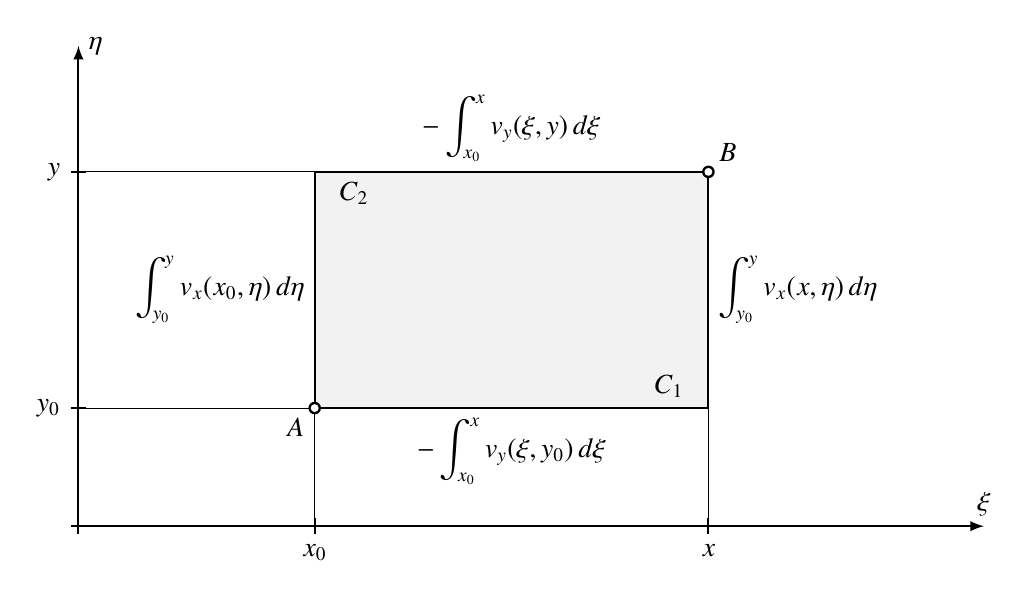
\begin{tikzpicture}[thick, >= latex]

\coordinate (A) at (0,0);
\coordinate (B) at (5,3);

\fill[color=gray!10] (A)--(5,0)--(B)--(0,3)--cycle;

\draw[line width=0.3pt] (0,-1.5)--(0,0);
\draw[line width=0.3pt] (-3,0)--(0,0);
\draw[line width=0.3pt] (5,-1.5)--(5,0);
\draw[line width=0.3pt] (-3,3)--(0,3);

\draw (0,-1.6)--(0,-1.4);
\node at (0,-1.6) [below] {$x_0$};
\draw (5,-1.6)--(5,-1.4);
\node at (5,-1.6) [below] {$x$};

\draw (-3.1,0)--(-2.9,0);
\node at (-3.1,0) [left] {$y_0$};
\draw (-3.1,3)--(-2.9,3);
\node at (-3.1,3) [left] {$y$};

\draw (A)--(5,0)--(B)--(0,3)--cycle;
\fill (A) circle[radius=0.08];
\fill[color=white] (A) circle[radius=0.05];
\fill (B) circle[radius=0.08];
\fill[color=white] (B) circle[radius=0.05];

\node at (A) [below left] {$A$};
\node at (B) [above right] {$B$};

\node at (4.5,0) [above] {$C_1$};
\node at (0.5,3) [below] {$C_2$};

\node at (2.5,0) [below] {$\displaystyle
-\int_{x_0}^x v_y(\xi,y_0)\,d\xi
$};

\node at (2.5,3) [above] {$\displaystyle
-\int_{x_0}^x v_y(\xi,y)\,d\xi
$};

\node at (0,1.5) [left] {$\displaystyle
\int_{y_0}^y v_x(x_0,\eta)\,d\eta
$};

\node at (5,1.5) [right] {$\displaystyle
\int_{y_0}^y v_x(x,\eta)\,d\eta
$};

\draw[->,line width=0.7pt] (-3.1,-1.5)--(8.5,-1.5) coordinate[label={above:$\xi$}];
\draw[->,line width=0.7pt] (-3,-1.6)--(-3,4.6) coordinate[label={right:$\eta$}];


\end{tikzpicture}
\end{document}

